% \documentclass{article}

\documentclass{article}
%% \documentclass[twocolumn]{article}

\renewcommand{\familydefault}{\sfdefault} % Standardfont ändern auf Sans Serif (bny)

\usepackage[utf8x]{inputenc}
\usepackage[german]{babel} % Sprache umschalten /hat funktioniert bis auf Authors, bny 13.04.2016
\usepackage{tcolorbox}
\usepackage{xcolor}
\definecolor{chamois}{rgb}{1,.984314,.956863}  % RGB 255 247 231
\pagecolor{chamois}
\usepackage{geometry}
\usepackage{eurosym}
\geometry{verbose,a4paper,tmargin=10mm,bmargin=10mm,lmargin=10mm,rmargin=10mm}
\usepackage[T1]{fontenc}

\usepackage{multicol} % 20.04.2017 hinzugefügt, bny

%%% \usepackage{tikz}
%%% % \pagecolor{olive!50!yellow!50!white}

%% --> Hinweis, 11.08.2017, bny
%% --> Multicol ist nur zuständig für Spalten, die farbigen Kacheln werden mit tcolorbox gemacht
%% --> soll nur eine einspaltige Box eingefügt werden, wird multicol auskommandiert. (siehe Beschaffung)

\tcbuselibrary{skins}

\colorlet{xlightblue}{blue!5}

\newtcolorbox{beamerlikethm}[1]{
  title=#1,
  beamer,
  % colback=xlightblue,
  colframe=red!50,
  fonttitle=\bfseries,
  left=1mm,
  right=1mm,
  top=1mm,
  bottom=1mm,
  middle=1mm
}


\begin{document}
\pagestyle{empty}

%%% \begin{tikzpicture}[remember picture, overlay]
%%% \shade[left color=red!50,
%%% right color=green!50
%%% ] (current page.north west) rectangle (current page.south east);
%%% \end{tikzpicture}


%%%%%%%%%%%%%%%%%%%
%   Plandruck
%%%%%%%%%%%%%%%%%%%

\pagebreak
\raggedleft{\huge Plandruck} \hspace{8cm} 
\includegraphics[width=.3\linewidth]{Pictures/PGLogo.png} \quad 
\includegraphics[width=.07\linewidth]{Pictures/Logo_t.png}
% \centering{{\huge Plandruck}} \hspace{5cm} 
\includegraphics[width=.3\linewidth]{Pictures/LogoPG_RBS_Verbindet.jpg} \quad 
\includegraphics[width=.07\linewidth]{Pictures/Logo_t.png}

% \vspace{\baselineskip}

%%%% Box 1+2 in zwei Spalten

\begin{multicols}{2}

\begin{tcolorbox}[colback=blue!5,colframe=blue!40!black,title=Dokumente für den Plandruck selektieren]
\begin{itemize}
  \item[$\Longrightarrow$] Wechseln Sie in die Dokumentenablage in die Übersicht 'Dokumente'. 
  \item[$\Longrightarrow$] Selektieren Sie die benötigen Dokumente. Nehmen Sie die Filterfunktion und die Volltextsuche zur Hilfe.
  \item[$\Longrightarrow$] Überprüfen Sie mit dem Dokumentenkorb 
\includegraphics[height=12pt]{Icons/dk_korb_b.jpg} 'Auswahl anzeigen', ob Ihre Selektion stimmt.
  \item[$\Longrightarrow$] Kehren Sie zurück und löschen oder ergänzen Sie die Auswahl von Dokumenten mit 
\includegraphics[height=10pt]{Icons/checkbox_leer.jpg} - 
\includegraphics[height=10pt]{Icons/checkbox_markiert.jpg}.
	\item[$\Longrightarrow$] Klick auf 
\includegraphics[height=12pt]{Icons/dk_korb_b.jpg} 'Auswahl löschen' löscht sämtliche Dokumente aus dem Dokumentenkorb.
	\item[$\Longrightarrow$] Klick auf 
\includegraphics[height=12pt]{Icons/dk_drucken.jpg} startet den Dialog für den Plandruck.
\end{itemize}
\end{tcolorbox}


\begin{tcolorbox}[colback=blue!5,colframe=blue!40!black,title=Plandruck Dialogfenster]
\begin{itemize}
  \item[$\Longrightarrow$] Nach Klick auf 
\includegraphics[height=12pt]{Icons/dk_drucken.jpg} wird das erste von zwei Dialogfenster geöffnet.
  \item[$\Longrightarrow$] Nehmen Sie alle gewünschten Einstellungen vor und achten Sie auf die Pflichtfelder (*).
  \item[$\Longrightarrow$] Mit der Schaltfläche 'Weiter zu Empfängerdetails' respektive 'Zurück zu allgemeinen Angaben' können Sie zwischen den Dialogfenstern wechseln.
	\item[$\Longrightarrow$] Klick auf \includegraphics[height=10pt]{Icons/info_blau.jpg} zeigt Ihnen bei Spalten weitere Informationen an.
	\item[$\Longrightarrow$] Schliessen Sie den Planauftrag mit Klick auf die Schaltfläche 'Auftrag absenden' ab. Der Auftrag wird ausgelöst und die Mails verschickt.
\end{itemize}
\end{tcolorbox}

\end{multicols}

%%% HINWEISE %%%
%%% Hinweise in 1er Spalte

\begin{beamerlikethm}{Hinweise}
\begin{itemize}
  \item[$\Longrightarrow$] Weisen Sie den Druckauftrag einem Projekt*, sowie Teilprojekt/Objekt (Freitextfeld) zu.
  \item[$\Longrightarrow$] Reprozentrum*: Wählen Sie das gewünschte Reprozentrum aus und priorisieren Sie den Auftrag.
  \item[$\Longrightarrow$] Das Auslieferungsdatum wird automatisch in Abhängigkeit der Bestellzeit und der Priorisierung erstellt.
  \item[$\Longrightarrow$] Für die Lieferung können Sie einen Zweck definieren, sowie eine Frist für Rückmeldungen festlegen.
  \item[$\Longrightarrow$] Mitteilungen an die Empfänger und das Reprozentrum können hier hinterlegt werden. Beim Dialogfenster 'Empfängerdetails' können pro Empfänger individuelle Nachrichten erfasst werden.
	\item[$\Longrightarrow$] Die Beilagen lassen sich mit blauem Link öffnen, das Format wird auf Grund des PDFs automatisch eruiert. Sie können das Format anpassen, sowie die Endbearbeitung definieren.
	\item[$\Longrightarrow$] Empfängerdetails: Fügen Sie Empfänger einzelnt oder mittels hinterlegter Liste hinzu. Pro Person sind weitere Einstellungen möglich:
	\item[$\Longrightarrow$] Anzahl Exemplare, Wahl Druckexemplar oder/und elektronisch. Selektieren Sie die gewünschten Beilagen (Lieferschein, Kontrollblatt). Können die Planlieferungen weiterverrechnet werden? Im Hintergrund wird ein Excel mit Angaben zur Verrechnung erstellt.
	\item[$\Longrightarrow$] Erfassung individueller Nachrichten, sowie entfernen eines Empfängers. Auftrag mit 'Auftrag absenden'.
\end{itemize}
\end{beamerlikethm}


%%%% Box 3+4 in zwei Spalten

\begin{multicols}{2}

\begin{tcolorbox}[colback=blue!5,colframe=blue!40!black,title=Druckaufträge Übersicht]
\begin{itemize}
  \item[$\Longrightarrow$] Wählen Sie den Menüpunkt 'Dokumentenablage' und den Unterpunkt 'Druckaufträge'.
  \item[$\Longrightarrow$] Sie erhalten eine Übersicht der Durckaufträge. Klick auf Nummer öffnet Detailansicht. Herunterladen des Lieferscheins sowie der versendeten Dokumenten möglich.
  \item[$\Longrightarrow$] Klick auf \euro{-Zeichen} öffnet die Verrechnungstabelle im Excel. Passen Sie die Daten an, auf dem Blatt 'Zusammenfassung' erscheint die Übersicht.
  \item[$\Longrightarrow$] Auf der 'persönlichen Projektübersicht' sehen Sie ebenfalls die pendenten sowie abgeschlossenen Druckaufträge. Sobald ein Reprozentrum Auftrag ausgeührt hat, werden die Angaben aktualisiert. 
\end{itemize}
\end{tcolorbox}


\begin{tcolorbox}[colback=blue!5,colframe=blue!40!black]

\begin{centering}
\center{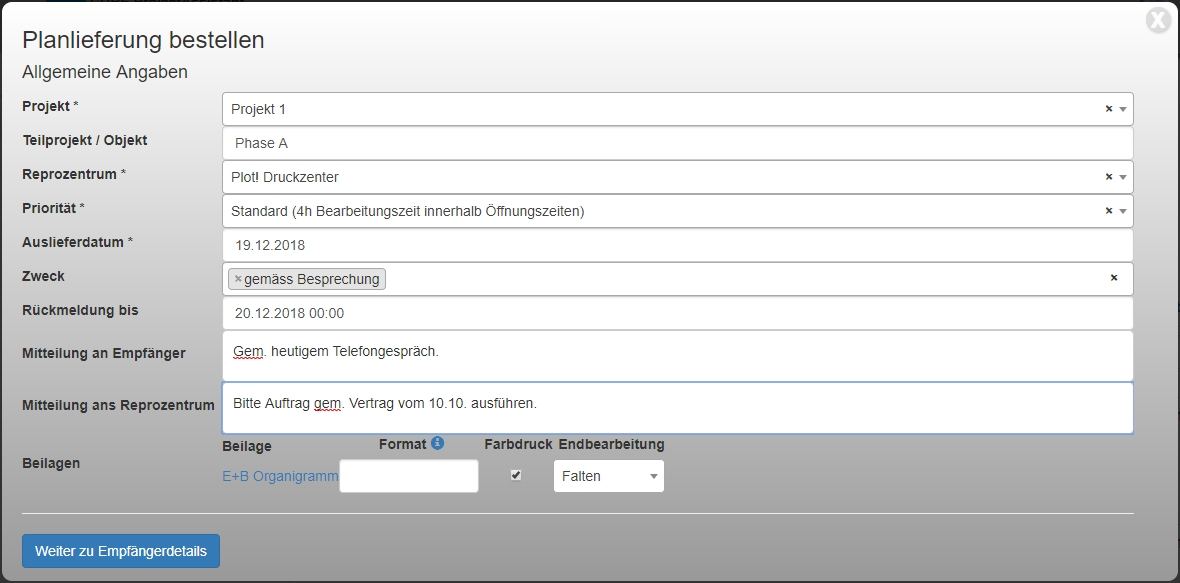
\includegraphics[width=1\linewidth]{Pictures/PlanDruck1.jpg}}
\end{centering}

\begin{centering}
\vspace{-15pt}
\center{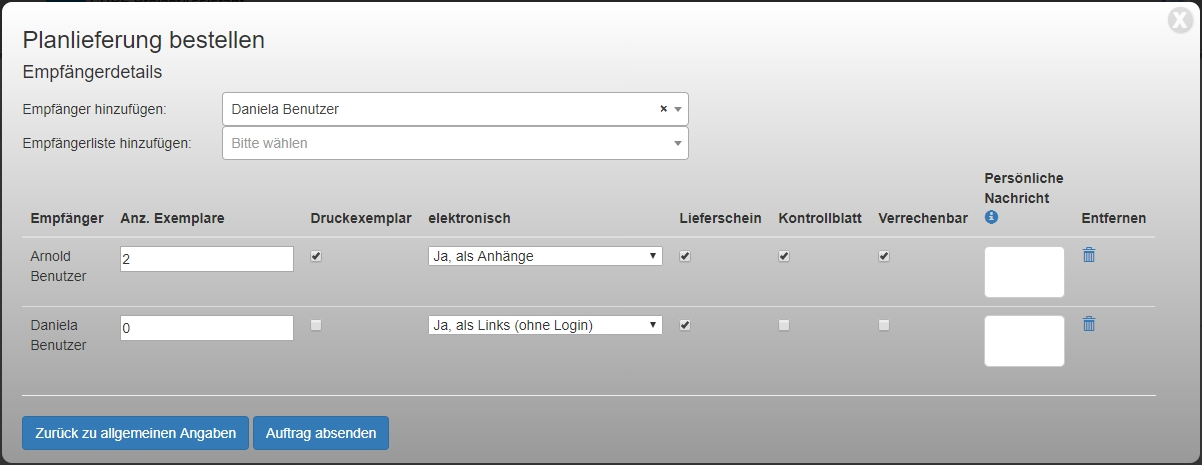
\includegraphics[width=1\linewidth]{Pictures/PlanDruck2.jpg}}
\end{centering}

\end{tcolorbox}
\end{multicols}

\end{document}